% Hlavicka pro protokoly z fyzikalniho praktika.
% Verze pro: LaTeX
% Verze hlavicky: 22. 2. 2007
% Autor: Ustav fyziky kondenzovanych latek
% Ke stazeni: www.physics.muni.cz/ufkl/Vyuka/
% Licence: volne k pouziti, nejlepe k vcasnemu odevzdani protokolu z Vaseho mereni.


\documentclass[czech,11pt,a4paper]{article}
\usepackage[T1]{fontenc}
\usepackage{graphicx}
\usepackage{mathtools}
\usepackage{amssymb}
\usepackage{amsthm}
\usepackage{thmtools}
\usepackage{xcolor}
\usepackage{nameref}
\usepackage{babel}
\usepackage{hyperref}
\usepackage{multicol}
\usepackage[export]{adjustbox}
\usepackage{subcaption}
\usepackage{caption}
\usepackage{multirow}
\usepackage{float}
\usepackage{placeins}




%%% Nemente:
\usepackage[margin=2cm]{geometry}
\newtoks\jmenopraktika \newtoks\jmeno \newtoks\datum
\newtoks\obor \newtoks\skupina \newtoks\rocnik \newtoks\semestr
\newtoks\cisloulohy \newtoks\jmenoulohy
\newtoks\tlak \newtoks\teplota \newtoks\vlhkost
%%% Nemente - konec.


%%%%%%%%%%% Doplnte pozadovane polozky:

\jmenopraktika={Fyzikální praktikum 2}  % nahradte jmenem vaseho predmetu
\jmeno={Teodor Duraković}            % nahradte jmenem mericiho
\datum={4.~listopadu 2024}        % nahradte datem mereni ulohy
\obor={F}                     % nahradte zkratkou vami studovaneho oboru
\skupina={Po 14:00}            % nahradte dobou vyuky vasi seminarni skupiny
\rocnik={II}                  % nahradte rocnikem, ve kterem studujete
\semestr={III}                 % nahradte semestrem, ve kterem studujete

\cisloulohy={5}               % nahradte cislem merene ulohy
\jmenoulohy={Magnetické pole} % nahradte jmenem merene ulohy

\tlak={1001}                   % nahradte tlakem pri mereni (v hPa)
\teplota={22.6}               % nahradte teplotou pri mereni (ve stupnich Celsia)
\vlhkost={40}               % nahradte vlhkosti vzduchu pri mereni (v %)

%%%%%%%%%%% Konec pozadovanych polozek.


%%%%%%%%%%% Uzitecne balicky:

%%%%%% Zamezeni parchantu:
\widowpenalty 10000 \clubpenalty 10000 \displaywidowpenalty 10000
%%%%%% Parametry pro moznost vsazeni vetsiho poctu obrazku na stranku
\setcounter{topnumber}{3}	  % max. pocet floatu nahore (specifikace t)
\setcounter{bottomnumber}{3}	  % max. pocet floatu dole (specifikace b)
\setcounter{totalnumber}{6}	  % max. pocet floatu na strance celkem
\renewcommand\topfraction{0.9}	  % max podil stranky pro floaty nahore
\renewcommand\bottomfraction{0.9} % max podil stranky pro floaty dole
\renewcommand\textfraction{0.1}	  % min podil stranky, ktery musi obsahovat text
\intextsep=8mm \textfloatsep=8mm  %\intextsep pro ulozeni [h] floatu a \textfloatsep pro [b] or [t]

% Tecky za cisly sekci:
\renewcommand{\thesection}{\arabic{section}.}
\renewcommand{\thesubsection}{\thesection\arabic{subsection}.}
\renewcommand{\thesubsubsection}{\thesubsection\arabic{subsubsection}.}
% Jednopismenna mezera mezi cislem a nazvem kapitoly:
\makeatletter \def\@seccntformat#1{\csname the#1\endcsname\hspace{1ex}} \makeatother


%%%%%%%%%%%%%%%%%%%%%%%%%%%%%%%%%%%%%%%%%%%%%%%%%%%%%%%%%%%%%%%%%%%%%%%%%%%%%%%
%%%%%%%%%%%%%%%%%%%%%%%%%%%%%%%%%%%%%%%%%%%%%%%%%%%%%%%%%%%%%%%%%%%%%%%%%%%%%%%
% Zacatek dokumentu
%%%%%%%%%%%%%%%%%%%%%%%%%%%%%%%%%%%%%%%%%%%%%%%%%%%%%%%%%%%%%%%%%%%%%%%%%%%%%%%
%%%%%%%%%%%%%%%%%%%%%%%%%%%%%%%%%%%%%%%%%%%%%%%%%%%%%%%%%%%%%%%%%%%%%%%%%%%%%%%

\begin{document}
	
	%%%%%%%%%%%%%%%%%%%%%%%%%%%%%%%%%%%%%%%%%%%%%%%%%%%%%%%%%%%%%%%%%%%%%%%%%%%%%%%
	% Nemente:
	%%%%%%%%%%%%%%%%%%%%%%%%%%%%%%%%%%%%%%%%%%%%%%%%%%%%%%%%%%%%%%%%%%%%%%%%%%%%%%%
	\thispagestyle{empty}
	
	{
		\begin{center}
			\sf 
			{\Large Ústav fyzikální elektroniky Přírodovědecké fakulty Masarykovy univerzity} \\
			\bigskip
			{\huge \bfseries FYZIKÁLNÍ PRAKTIKUM} \\
			\bigskip
			{\Large \the\jmenopraktika}
		\end{center}
		
		\bigskip
		
		\sf
		\noindent
		\setlength{\arrayrulewidth}{1pt}
		\begin{tabular*}{\textwidth}{@{\extracolsep{\fill}} l l}
			\large {\bfseries Zpracoval:}  \the\jmeno & \large  {\bfseries Naměřeno:} \the\datum\\[2mm]
			\large  {\bfseries Obor:} \the\obor  \hspace{40mm}  {\bfseries Skupina:} \the\skupina %
			%{\bfseries Ročník:} \the\rocnik \hspace{5mm} {\bfseries Semestr:} \the\semestr  
			&\large {\bfseries Testováno:}\\
			\\
			\hline
		\end{tabular*}
	}
	
	\bigskip
	
	{
		\sf
		\noindent \begin{tabular}{p{3cm} p{0.6\textwidth}}
			\Large  Úloha č. {\bfseries \the\cisloulohy:} \par
			\smallskip
			$T=\the\teplota$~$^\circ$C \par
			$p=\the\tlak$~hPa \par
			$\varphi=\the\vlhkost$~\%
			&\Large \bfseries \the\jmenoulohy  \\[2mm]
		\end{tabular}
	}
	
	\vskip1cm
	
	%%%%%%%%%%%%%%%%%%%%%%%%%%%%%%%%%%%%%%%%%%%%%%%%%%%%%%%%%%%%%%%%%%%%%%%%%%%%%%%
	% konec Nemente.
	%%%%%%%%%%%%%%%%%%%%%%%%%%%%%%%%%%%%%%%%%%%%%%%%%%%%%%%%%%%%%%%%%%%%%%%%%%%%%%%
	
	%%%%%%%%%%%%%%%%%%%%%%%%%%%%%%%%%%%%%%%%%%%%%%%%%%%%%%%%%%%%%%%%%%%%%%%%%%%%%%%
	%%%%%%%%%%%%%%%%%%%%%%%%%%%%%%%%%%%%%%%%%%%%%%%%%%%%%%%%%%%%%%%%%%%%%%%%%%%%%%%
	% Zacatek textu vlastniho protokolu
	%%%%%%%%%%%%%%%%%%%%%%%%%%%%%%%%%%%%%%%%%%%%%%%%%%%%%%%%%%%%%%%%%%%%%%%%%%%%%%%
	%%%%%%%%%%%%%%%%%%%%%%%%%%%%%%%%%%%%%%%%%%%%%%%%%%%%%%%%%%%%%%%%%%%%%%%%%%%%%%%
	
	\begin{multicols}{2}
	\section{Zadání}
	1. Změřit horizontální složku intenzity magnetického pole Země Gaussovým magnetometrem.\\
	2. Zjistit magnetickou odezvu feromagnetického materiálu.
	\section{Úvod}
	\subsection{Geomagnetické pole}
	Znalost průběhu magnetického pole v okolí Země je důležitá pro mnoho oborů, jako je například geografie, geologie a podobně. Vlastnosti magnetického pole Země popisuje intenzita magnetického pole, obvykle značená $\boldsymbol{H}$. V každém bodě můžeme vektor intenzity rozdělit na horizontální a vertikální složku, v dalším se soustředíme jen na měření horizontální složky $H_{z}$.
	
	Princip metody měření Gaussovým magnetometrem spočívá v porovnání intenzity zemského magnetického pole s intenzitou tyčového permanentního magnetu pomocí magnetické střelky jako detektoru směru lokálního magnetického pole. Z praktických důvodů se v metodě provádí měření výchylky magnetické střelky pro dvě polohy střelky vzhledem k permanentnímu magnetu, pro tzv. první a druhou Gaussovu polohu (viz obr. 1).
	
	Pro výpočet intenzity magnetického pole od tyčového magnetu použijeme vztah pro magnetické pole v okolí magnetického dipólu s dipólovým momentem $\boldsymbol{m}$
	$$
	\boldsymbol{H}(\boldsymbol{r})=\frac{1}{4 \pi \mu_{0} r^{3}}\left[\frac{3(\boldsymbol{r} \cdot \boldsymbol{m}) \boldsymbol{r}}{r^{2}}-\boldsymbol{m}\right]
	$$
	kde $\boldsymbol{r}$ je polohový vektor bodu v němž počítáme magnetické pole vzhledem k poloze magnetického dipólu a $\mu_{0}$ je permeabilita vakua. V reálném případě se ovšem rozměry permanentního magnetu vzhledem ke vzdálenosti, ve které měříme, nedají zanedbat. Proto je třeba tento vztah integrovat přes celý magnet s danou objemovou hustotou dipólového momentu.
	
	Integrace pro první Gaussovu polohu, tj. případ střelky na ose tyčového magnetu, vede na výsledek
	\begin{equation}
		H_{1}(r)  =\frac{1}{2 \pi \mu_{0} r^{3}} \frac{M}{\left(1-\lambda^{2}\right)^{2}}
	\end{equation}
	kde $\mu=M / l$ je délková hustota magnetického momentu, $\lambda=l / 2 r, r$ je vzdálenost mezi osou magnetické střelky a středem (těžištěm) tyčového magnetu a $l$ je délka tyčového magnetu s celkovým magnetickým momentem $M$. Zde jsme aproximovali válcový tyčový magnet nekonečně tenkou tyčí. Konečný průměr magnetu se v praxi projeví tím, že veličina $l$ ve vztahu (1) neodpovídá jeho fyzické, ale tzv. redukované délce. \end{multicols}
	\begin{figure}[H]
	\begin{center}
		
		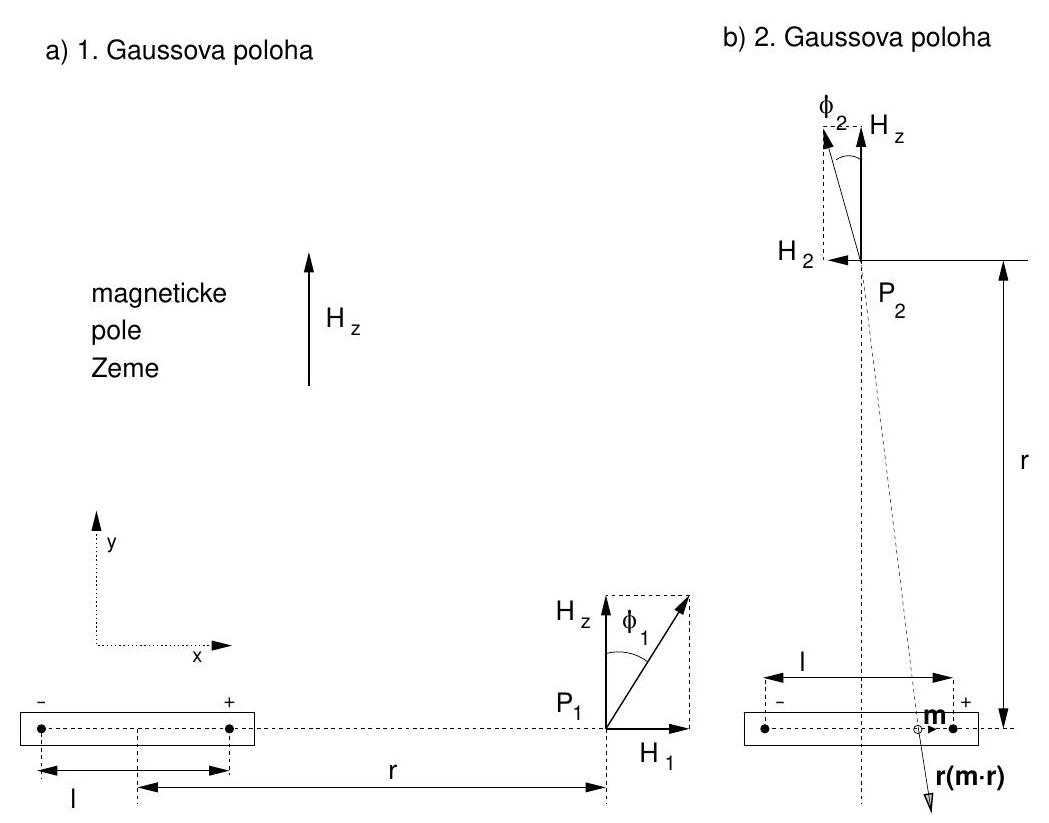
\includegraphics[width=0.6\linewidth, ]{Gaussovypolohy} 
		\caption{Znázornění 1. a 2. Gaussovy polohy, přičemž }
	\end{center}
	
	\end{figure} 
	
	\begin{multicols}{2}
	V druhé Gaussově poloze se sice směr pole vyvolaného různými elementy podél délky tyčového magnetu mění, ale vzhledem k symetrii se složka ve směru kolmém na osu magnetu vyruší. Počítat tedy budeme pouze komponentu ve směru osy tyčového magnetu (zde osa $x$ ). Integrací pak dospějeme ke vztahu:
	
	\begin{equation}
		H_{2}(r) =-\frac{1}{4 \pi \mu_{0} r^{3}} \frac{M}{\left(1+\lambda^{2}\right)^{3 / 2}}
	\end{equation}
	
	Známe tedy intenzitu magnetického pole v bodech $\mathrm{P}_{1}$ a $\mathrm{P}_{2}$. Umístíme magnet tak, aby jeho osa směřovala kolmo ke směru magnetického pole Země. Výchylka magnetky v první Gaussově poloze z jejího původního směru k magnetickému pólu Země je $\varphi_{1}$, přičemž platí
	\begin{equation}
		\tan \varphi_{1}=\frac{H_{1}}{H_{z}}=\frac{1}{4 \pi \mu_{0} H_{z}} \frac{2 M}{r^{3}\left(1-\lambda^{2}\right)^{2}}
	\end{equation}
	Obdobně v místě $\mathrm{P}_{2}$ se střelka vychýlí o úhel $\varphi_{2}$
	
\begin{equation}
		\tan \varphi_{2}=\frac{H_{2}}{H_{z}}=\frac{1}{4 \pi \mu_{0} H_{z}} \frac{M}{r^{3}\left(1+\lambda^{2}\right)^{3 / 2}}
\end{equation}
	Úpravou rovnic získáváme vztahy 
	\begin{gather}
		\frac{M}{H_{z}}=\frac{4 \pi \mu_{0} r^{3}}{7}\left(\frac{3 \tan \varphi_{1}}{2}+4 \tan \varphi_{2}\right)\\
		M H_{z}=\frac{\pi^{2} J}{\tau^{2}},
	\end{gather}
	kde $J$ je Moment setrvačnosti magnetu daný vztahem
	\begin{equation}
		J=\frac{m}{4}\left(R^{2}+\frac{l^{2}}{3}\right),
	\end{equation}
	kde $m$ je hmotnost magnetu, $R$ jeho poloměr a $l$ délka.
	$\tau$ je polovina periody kmitů magnetu v tíhovém poli závislá na horizontální složce magnetické intenzity Země, hodnotu periody získáme zavěšením magnetu na vlákno o malém torzním momentu, čímž je torze ovlivněna právě magnetickým polem Země.
	
	\begin{equation}
		\tau = \frac T 2
	\end{equation}
	Vztahy (5), (6) nám udávají veličiny $A=M / H_{z}$ a $B=M H_{z}$. Z těchto veličin určíme velikost horizontální složky intenzity magnetického pole Země jako
	
	\begin{equation}
		H_{z}=\sqrt{\frac{B}{A}}
	\end{equation}
	\subsection{Magnetická odezva feromagnetického materiálu}
	Vztah mezi magnetickou intenzitou $\boldsymbol{H}$ a magnetickou indukcí $\boldsymbol{B}$ je dán vztahem
	
\begin{equation}
		\boldsymbol{B}=\mu_{0}(\boldsymbol{H}+\boldsymbol{M}),
\end{equation}
	
	kde $\boldsymbol{M}$ je vektor magnetizace, který udává objemovou hustotu magnetického momentu. V případě paramagnetických a diamagnetických materiálů ve slabém magnetickém poli můžeme závislost magnetizace na okolním poli předpokládat v lineárním tvaru
	
\begin{equation}
		\boldsymbol{M}=\chi \mu_{0} \boldsymbol{H}
\end{equation}
	kde $\chi$ je magnetická susceptibilita, která je kladná pro paramagnetické a záporná pro diamagnetické materiály. Pro většinu materiálů, s výjimkou přechodových kovů a jejich sloučenin, je susceptibilita velmi malá, okolo $10^{-6}$ až $10^{-9}$. Zřejmě též platí $\boldsymbol{B}=(1+\chi) \mu_{0} \boldsymbol{H}=\mu_{r} \mu_{0} \boldsymbol{H}$, kde $\mu_{r}$ je relativní permeabilita. V obecném případě je susceptibilita tenzorem a vektory magnetizace a intenzity nemusejí mít stejný směr. Pro feromagnetické materiály však není závislost magnetické indukce na intenzitě pole lineární a vykazuje hysterezní závislost, jejíž typický průběh je znázorněn na obrázku 2.
		\begin{figure}[H]
		\begin{center}
			
			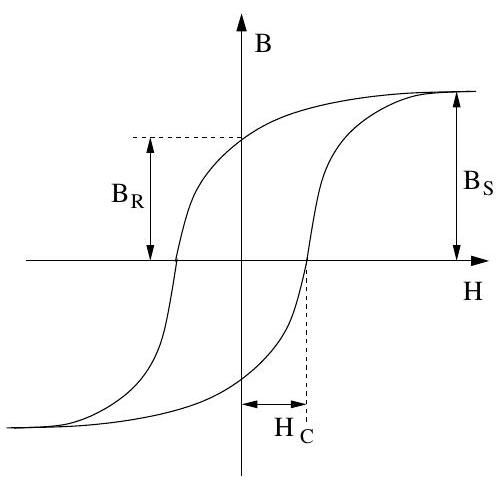
\includegraphics[width=0.9\linewidth, ]{SmyckaT} 
			\caption{Typický průběh magnetické hysterezní smyčky }
		\end{center}
		
	\end{figure} 
	Měření budeme provádět na feromagnetickém jádře se dvěma vinutími (transformátoru) buzeném střídavým elektrickým proudem zapojeném podle schématu na obrázku 3 Primární vinutí slouží k buzení magnetického pole a na sekundárním snímáme indukované napětí. Intenzitu
		\begin{figure}[H]
		\begin{center}
			
			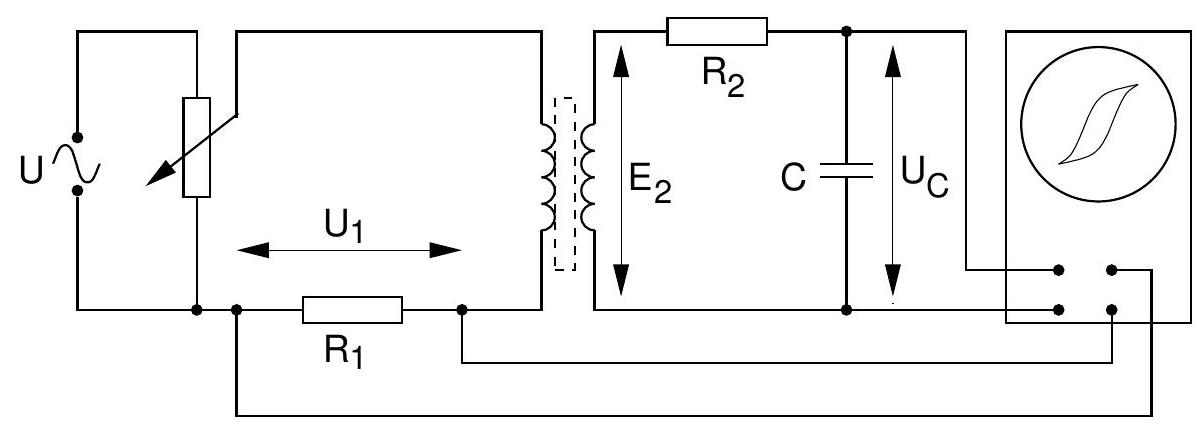
\includegraphics[width=0.9\linewidth, ]{Zapojeni} 
			\caption{Schéma obvodu pro měření magnetického pole ve feromagnetu}\end{center}		
	\end{figure} 
	Intenzitu magnetického pole můžeme spočíst podle Ampérova zákona
	
\begin{equation}
		\oint_{L} \boldsymbol{H} \cdot \mathrm{~d} \boldsymbol{l}=\int_{S} \boldsymbol{j} \cdot \boldsymbol{n} \mathrm{~d} S,
\end{equation}
	kde integrace na levé straně probíhá podél uzavřené křivky $L$, na pravé straně přes plochu $S_{1}$ jí ohraničenou a $\boldsymbol{j}$ je proudová hustota tekoucí plochou (výsledkem integrace pravé strany je zde celkový proud protékající vodiči uvnitř kružnice). V případě toroidu je řešení jednoduché. Integraci provedeme podél kružnice s poloměrem $r$.
	Z důvodu symetrie má intenzita $H$ podél kružnice všude stejnou velikost a předchozí rovnice pak přejde do tvaru
	
\begin{equation}
		2 \pi r H=N_{1} I, \quad H=\frac{N_{1} I}{2 \pi r},
\end{equation}
	
	kde $N_{1}$ je počet závitů primárního vinutí a $I$ proud tekoucí každým z nich. Magnetická intenzita je tedy přímo úměrná proudu, který měříme jako napětí $U_{1}$ na rezistoru $R_{1}$ připojeném do série s proudovou cívkou. Hodnota magnetické intenzity v toroidu je rovna
	
\begin{equation}
		H(t)=\frac{N_{1}}{2 \pi r R_{1}} U_{1}(t)
\end{equation}
	
	
	Pokud je rozdíl vnitřního a vnějšího poloměru dostatečně malý, můžeme považovat hodnotu magnetické intenzity nezávislou na poloze v toroidu a za poloměr $r$ dosadit jeho průměrnou hodnotu $r=\left(r_{\text {min }}+r_{\text {max }}\right) / 2$.
	
	Při buzení střídavým proudem se mění s časem též magnetická indukce. Časová změna magnetické indukce $B$ indukuje v sekundárním vinutí elektromotorické napětí $E_{2}$ podle Faradayova zákona
	
\begin{equation}
		E_{2}(t)=-\frac{\mathrm{d} \Phi}{\mathrm{~d} t}=-N_{2} S_{2} \frac{\mathrm{~d} B}{\mathrm{~d} t}
\end{equation}
	
	kde $\Phi$ je celkový magnetický tok sekundární cívkou; vycházíme z toho, že je-li průřez jádra toroidu $S_{2}$ a počet závitů sekundárního vinutí $N_{2}$, pak magnetický tok je roven $\Phi=N_{2} S_{2} B$. Indukované napětí je úměrné časové změně magnetické indukce. Abychom mohli měřit přímo napětí úměrné magnetické indukci, je v obvodu zařazen integrační RC člen. Průběh napětí na kondenzátoru o kapacitě $C$ získáme z druhého Kirchhoffova zákona
\begin{equation}
		E_{2}=R I_{2}+U_{C}, \quad U_{C}=\frac{Q}{C}, \quad I_{2}=\frac{\mathrm{d} Q}{\mathrm{~d} t}
\end{equation}
	
	kde $I_{2}$ je proud tekoucí obvodem a $Q$ je náboj na kondenzátoru. Po úpravě získáme diferenciální rovnici pro náboj $Q$
\begin{equation}
		\frac{\mathrm{d} Q}{\mathrm{~d} t}+\frac{Q}{R C}=\frac{1}{R} E_{2}(t)
\end{equation}
	Tato rovnice má řešení ve tvaru
	\begin{equation}
		Q(t)=-\frac{1}{R} \int_{0}^{\infty} E_{2}(t-\tau) \mathrm{e}^{-\frac{\tau}{R C}} \mathrm{~d} \tau
	\end{equation}
	
	
	Průběh napětí na kondenzátoru je potom dán vztahem
	\begin{equation}
		U_{C}(t)=-\frac{1}{R C} \int_{0}^{\infty} E_{2}(t-\tau) \mathrm{e}^{-\frac{\tau}{R C}} \mathrm{~d} \tau
	\end{equation}
	
	Je-li časová konstanta integračního obvodu $R C$ mnohem větší než perioda budícího střídavého proudu, lze exponenciální člen v integrálu položit přibližně roven 1 . Potom po dosazení z rovnice (15) do vztahu (19) dostaneme výraz pro napětí $U_{C}$
	
\begin{equation}
		\left.U_{C}(t) \approx \frac{1}{R C} \int_{-\infty}^{t} N_{2} S_{2} \frac{\mathrm{~d} B}{\mathrm{~d} t}\right|_{\tau} \mathrm{d} \tau, \quad U_{C}(t) \approx \frac{N_{2} S_{2}}{R C} B(t)
\end{equation}
	
	
	Po převedení dostaneme vztah pro magnetickou indukci
	
\begin{equation}
		B(t)=\frac{R C}{N_{2} S_{2}} U_{C}(t)
\end{equation}
	
	
	V zapojení podle schématu na obrázku 3 nastavíme osciloskop do tzv. X-Y režimu, kdy zobrazujeme vzájemnou závislost napětí na jednotlivých vstupech. Jelikož podle vztahu (14) je napětí na prvním vstupu úměrné intenzitě magnetického pole a napětí na druhém vstupu je podle vztahu (21) úměrné indukci magnetického pole, zobrazujeme přímo hysterezní smyčku, tedy závislost indukce na intenzitě magnetického pole. Napětí naměřená na osciloskopu pak již převedeme na indukci a intenzitu magnetického pole ve zvolených bodech hysterezní smyčky pomocí výše zmíněných vztahů 14 a 16.
		
	Magnetizaci můžeme snadno spočíst z magnetické indukce s použitím vztahu (5.22) jako
	
\begin{equation}
		M=\frac{B}{\mu_{0}}-H
\end{equation}
	

	\section{Měření}
	\subsection{Geomagnetické pole}
	Měřením získáváme rozměry, hmotnost a periodu kmitů magnetu:
	\begin{gather*}
		l = 123.78 \pm 0.19 \,\mathrm{mm}\\ r = 10.6 \pm 0.3 \,\mathrm{mm}\\ m = 298.3 \pm 0.3  \,\mathrm{g} \\ T = 5.12 \pm 0.06 \,\mathrm{s}
	\end{gather*}
	a pro jednotlivé Gaussovy polohy získáváme výchylky
	
	\begin{center}
		\begin{tabular}{|c|c|c|}
		\hline
		$r$ [cm] & $\varphi\, [^\circ]$ & $\varphi ^\prime\, [^\circ]$ \\ \hline
		-40    & 55        & 50                \\ \hline
		-30    & 75        & 70                \\ \hline
		-20    & 85        & 85                \\ \hline
		20     & 85        & 85                \\ \hline
		30     & 75        & 75                \\ \hline
		40     & 55        & 55                \\ \hline
	\end{tabular}\\
	\end{center}
	pro I. Gaussovu polohu a \\
\begin{center}
		\begin{tabular}{|c|c|c|}
		\hline
		r [cm] & $\varphi_2\, [^\circ]$ & $\varphi_2 ^\prime\, [^\circ]$ \\ \hline
		-40    & 37        & 30                \\ \hline
		-30    & 55        & 47                \\ \hline
		-20    & 80        & 75                \\ \hline
		20     & 78        & 82                \\ \hline
		30     & 60        & 50                \\ \hline
		40     & 40        & 30                \\ \hline
	\end{tabular}\\
\end{center}
	pro II. Gaussovu polohu.
	Pro hodnoty A získáváme
	\begin{center}
		\begin{tabular}{|c|c|}
		\hline
		r [cm] & $A . 10^{-7}[\mathrm{Hm^2}]$ \\ \hline
		-40    &$ 6.6  \pm 0.6 $                     \\ \hline
		-30    &$ 5.9 \pm    0.6    $                 \\ \hline
		-20    &$ 6.4 \pm       0.7    $              \\ \hline
		20     &$ 7.2 \pm    0.8      $               \\ \hline
		30     & $6.9 \pm    0.6      $               \\ \hline
		40     &$ 7.1 \pm    0.8      $               \\ \hline
	\end{tabular}
	\end{center}
	\begin{equation}
		A = (6.69 \pm 0.3 ).10^{-7} \,\mathrm{H. m^2}
	\end{equation}
	Pro B získáváme
	\begin{equation}
		B = (1.47 \pm 0.04).10^{-4} \,\mathrm{kg\, m^2\, s^{-2}}
	\end{equation}
	proto 
	\begin{equation}
		H_z = 14.8 \pm 0.4 \,\mathrm{A\,m^{-1}} = 18600 \pm 500 \,\mathrm{nT}
	\end{equation}
	Získané hodnoty, přestože řádově korektní, se od udávaných hodnot viditelně liší. Tuto deviaci můžeme vysvětlit zejména nemožností odečítat z kompasu přesnější hodnoty, což bylo limitováno zejména samotnou škálou kompasu.
	\subsection{Magnetická odezva feromagnetického materiálu}
	Změřené dimenze toroidu jsou:
	\begin{gather*}
		h = 7\,\mathrm{mm}\\
		r_{min} = 9.9\,\mathrm{mm}\\
		r_{max} = 14.85 \,\mathrm{mm}\\
		r = 12.378\,\mathrm{mm}\\
		S = 34.65\,\mathrm{mm^2}
	\end{gather*}
	Parametry komponent obvodu jsou:
	\begin{gather*}
		R_1 = 83 \,\mathrm{\Omega}\\
		R_2 = 120 \,\mathrm{k\Omega}\\
		N_1 = 260 \\
		N_2 = 900 \\
		C = 1.0 \,\mathrm{\mu F}
	\end{gather*}
 	Po zapojení dle obr. 3 získáváme následující hysterezní křivku a data:
 	\begin{figure}[H]
 		\begin{center}
 			
 			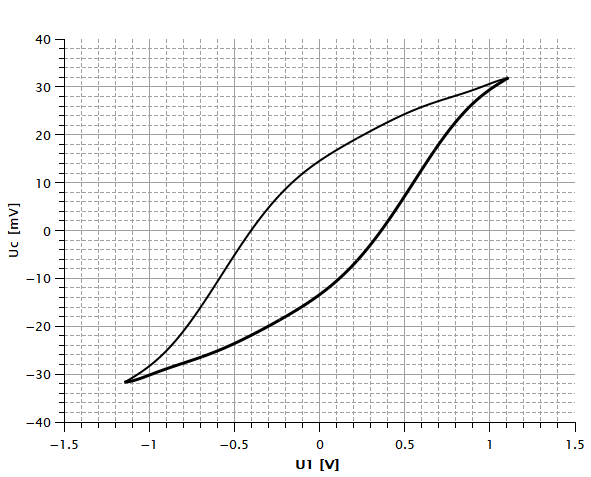
\includegraphics[width=0.9\linewidth, ]{hystereze} 
 			\caption{Získaná hysterezní smyčka}
 		\end{center} 		
 	\end{figure} 
 	\begin{gather*}
 		U_{1_S} = 1.127 \,\mathrm{V}\\
 		U_{1} = 0.382 \,\mathrm{V}\\
 		U_{C_{R}} = 0.014 \,\mathrm{V}\\
 		U_{C_{S}} = 0.032 \,\mathrm{V} 		
 	\end{gather*} 	
 	Prostřednictvím vztahu (14) získáme hodnotu magnetické intenzity:
 	\begin{gather*}
 		H_s = 45.39\,\mathrm{A.m^{-1}}\\
 		H_c = 15.39\,\mathrm{A.m^{-1}}
 	\end{gather*}
 	Vzorcem (21) zjistíme příslušné hodnoty magnetické indukce:
 	\begin{gather*}
 		B_R = 53.87 \,\mathrm{mT}\\
 		B_S = 123.14 \,\mathrm{mT}
 	\end{gather*}
 	A pomocí vztahu (22) určíme hodnotu magnetizace:
 	\begin{gather*}
 		M_R = 42.852 \,\mathrm{A/m}\\
 		M_S = 97.976 \,\mathrm{A/m}
 	\end{gather*}
 	
	\section{Závěr}
	Podařilo se nám splnit veškeré zadané úkoly a získat hodnoty hledaných veličin, přičemž jsme původcem nemalých odchylek v první úloze označili nedostatečně přesnou měřicí aparaturu a v jejím důsledku i naši sníženou přesnost odečítání získaných hodnot.
	
	
	
	
	
	
	
	% Nakonec nezapomeňte projet text programem vlna nebo vlnka, např.
	% 	vlna -m -l -n mojeuloha.tex
	% nebo zkontrolovat a opravit jednopísmenné předložky na koncích řádků ručně.
	\end{multicols}
\end{document}
